\documentclass[12pt,letterpaper]{article}

\usepackage{fullpage}
\usepackage[top=2cm, bottom=4.5cm, left=2.5cm, right=2.5cm]{geometry}
\usepackage{amsmath,amsthm,amsfonts,amssymb,amscd}
\usepackage{lastpage}
\usepackage{enumerate}
\usepackage{fancyhdr}
\usepackage{mathrsfs}
\usepackage{xcolor}
\usepackage{graphicx}
\usepackage{listings}
\usepackage{bm}
\usepackage[htt]{hyphenat}
\usepackage{hyperref}

\hypersetup{%
  colorlinks=true,
  linkcolor=blue,
  linkbordercolor={0 0 1}
}

\newtheorem*{thm}{Theorem}
 
\renewcommand\lstlistingname{Algorithm}
\renewcommand\lstlistlistingname{Algorithms}
\def\lstlistingautorefname{Alg.}

\lstdefinestyle{Python}{
    language        = Python,
    frame           = lines, 
    basicstyle      = \footnotesize,
    keywordstyle    = \color{blue},
    stringstyle     = \color{green},
    commentstyle    = \color{red}\ttfamily
}

\setlength{\parindent}{0.0in}
\setlength{\parskip}{0.12in}

% Edit these as appropriate
\newcommand\course{CSE 3500}
\newcommand\hwnumber{6}                  % <-- homework number

\pagestyle{fancyplain}
\headheight 35pt
\lhead{mfm19005}
\chead{\textbf{\Large Homework \hwnumber}}
\rhead{\course}
\lfoot{}
\cfoot{}
\rfoot{\small\thepage}
\headsep 1.5em

\begin{document}

\begin{center}
    \LARGE Competitive Analysis, Greedy and Graph Algorithms
\end{center}


\section*{Problem 0 -- Birthday Party! (40\%)}

In the typical algorithmic setup, we have complete information as input and a desired decision or optimization as output.
For example, given a weight graph, compute its maximum spanning tree.
Online algorithms are distinct from this typical setup and are used to model situations of incomplete or streaming data.
With incomplete information we cannot guarantee optimality, but, we can reason about an algorithm's effectiveness. 
This, as we learned in class, is referred to as \textit{competitive analysis}.

The Spring 2019 CSE3500 class is invited to Professor Derek's birthday party in a week's time at 1:00pm.
You can't think of a good enough excuse not to go, so you RSVP 'yes'.
During lunch time a week later, you realize that you forgot to get Derek a gift.
Panicking, you walk over to a fruit bin in the dining hall where you can grab kiwis or pineapples. 
Pineapples are ten times as heavy as kiwis, so your bag can hold either $40$ kiwis, $4$ pineapples, or any combination of the two that respect the bag constraints.

You do not know if Derek enjoys pineapples or kiwis.
But you do know that for each kiwi you bring, Derek will gain $K\geq 0$ joy; likewise, for each pineapple that you bring, Derek will gain $P \geq 0$ joy.

\newpage
\subsection*{Task 1}

Given that we do not know the exact parameters that will make Derek happiest, a strategy we could employ to ensure that he receives some joy from our selection would be to choose a proportional amount of each fruit in order to fill the bag. That way, there is a non-zero amount of each type of fruit that Derek might enjoy leaving a margin of error for the fruit Derek does enjoy.

$\hfill \break$
For this particular example, we can pick \textit{two pineapples} and \textit{twenty kiwis} as our proportional selection.

\subsection*{Task 2}

For the above algorithm we devised, the competitive ratio would be $2$. This is the case as the oracle would consider one of the fruits to have a $joy = 0$, whereas the other fruit would have an arbitrary non-zero joy value, $J$. Therefore, the oracle would only bring the fruit that would bring Derek $J$ joy. As such, regardless of the amount of the fruit brought, the ratio will always be 2.

\subsection*{Task 3}

\begin{lstlisting}
Opt(P, K):
    if P > 10K:
        n_p = 4
        n_k = 0
    else:
        n_p = 0
        n_k = 40
\end{lstlisting}

This solution is optimal since if $P > 10K$, then because $n_p = 1 \equiv n_k = 10$, we know that $n_p \cdot p > n_k \cdot k$. This remains true for the reverse, when $n_k \cdot k > n_p \cdot p$. In this way, the joy is maximized for the given constraints. 

\subsection*{Task 4}

If $k = 0$ and $p = 1$, then the oracle's algorithm would have $n_p = 4$ and $n_k = 0$. This would result in $n_p = 2$ and $n_k = 20$ and a joy value of four for the oracle's algorithm, and a value of two with our algorithm. In turn, this would generate a competitive ratio of 2.

\subsection*{Part 5a}

If $k, p$ are non-zero, then the oracle would receive $n_k = 0, n_p = 4$, while our algorithm would receive $n_k = 20, n_p = 2$. This would result in $\frac{(4 \cdot p) + (0 \cdot 0)}{(2 - k) + (20 \cdot 0)} = 2$. Thus, if both $k, p$ are non-zero, the oracle would get $n_k = 40, n_p = 0$. This would result in $\frac{(40 \cdot k) + (0 \cdot 0)}{(2 \cdot 0) + (20 \cdot k)} = 2$ and leave us with a competitive ratio of $2$.

\subsection*{Part 5b}

We know that the oracle's optimal solution for when $p > 10k$ is $n_p = 4, n_k = 0$, and our algorithm's solution is $n_k = 2, n_p = 20$. Therefore, we can conclude that any non-zero value of $n_k$ will increase the algorithm's total joy output, while not increasing the oracle's. In this way, we can tell that the greatest ratio will occur when $k = 0$. According to the results found in Part 5a, we can see that the competitive ratio would be two, which appears if $P > 10K$, and the oracle's inputs are $n_k = 40, n_p = 0$. Thus, the greatest ratio would be achieved when $p = 0$ which results in the desired competitive ratio of 2 (demonstrated in Part 5a).

\subsection*{Task 5c}

According to what we've gathered, we can see that the best algorithm would be $n_k = 20, n_p = 2$ since it would result in the best competitive ratio of two.

\newpage
\section*{Problem 1 -- Matryoshka dolls (30\%)}
Russian nesting dolls are wooden dolls of decreasing size in which the smaller dolls can be placed inside the larger dolls (Figure ~\ref{rnd}).
UConn happens to have the world's largest shadow economy dedicated to the buying and selling of nesting dolls. 
Professor Derek sees an economic opportunity and decides to plan an elaborate Russian nesting doll heist\footnote{Stealing is, in general, bad.}.

\begin{figure}[h!]
    \centering
    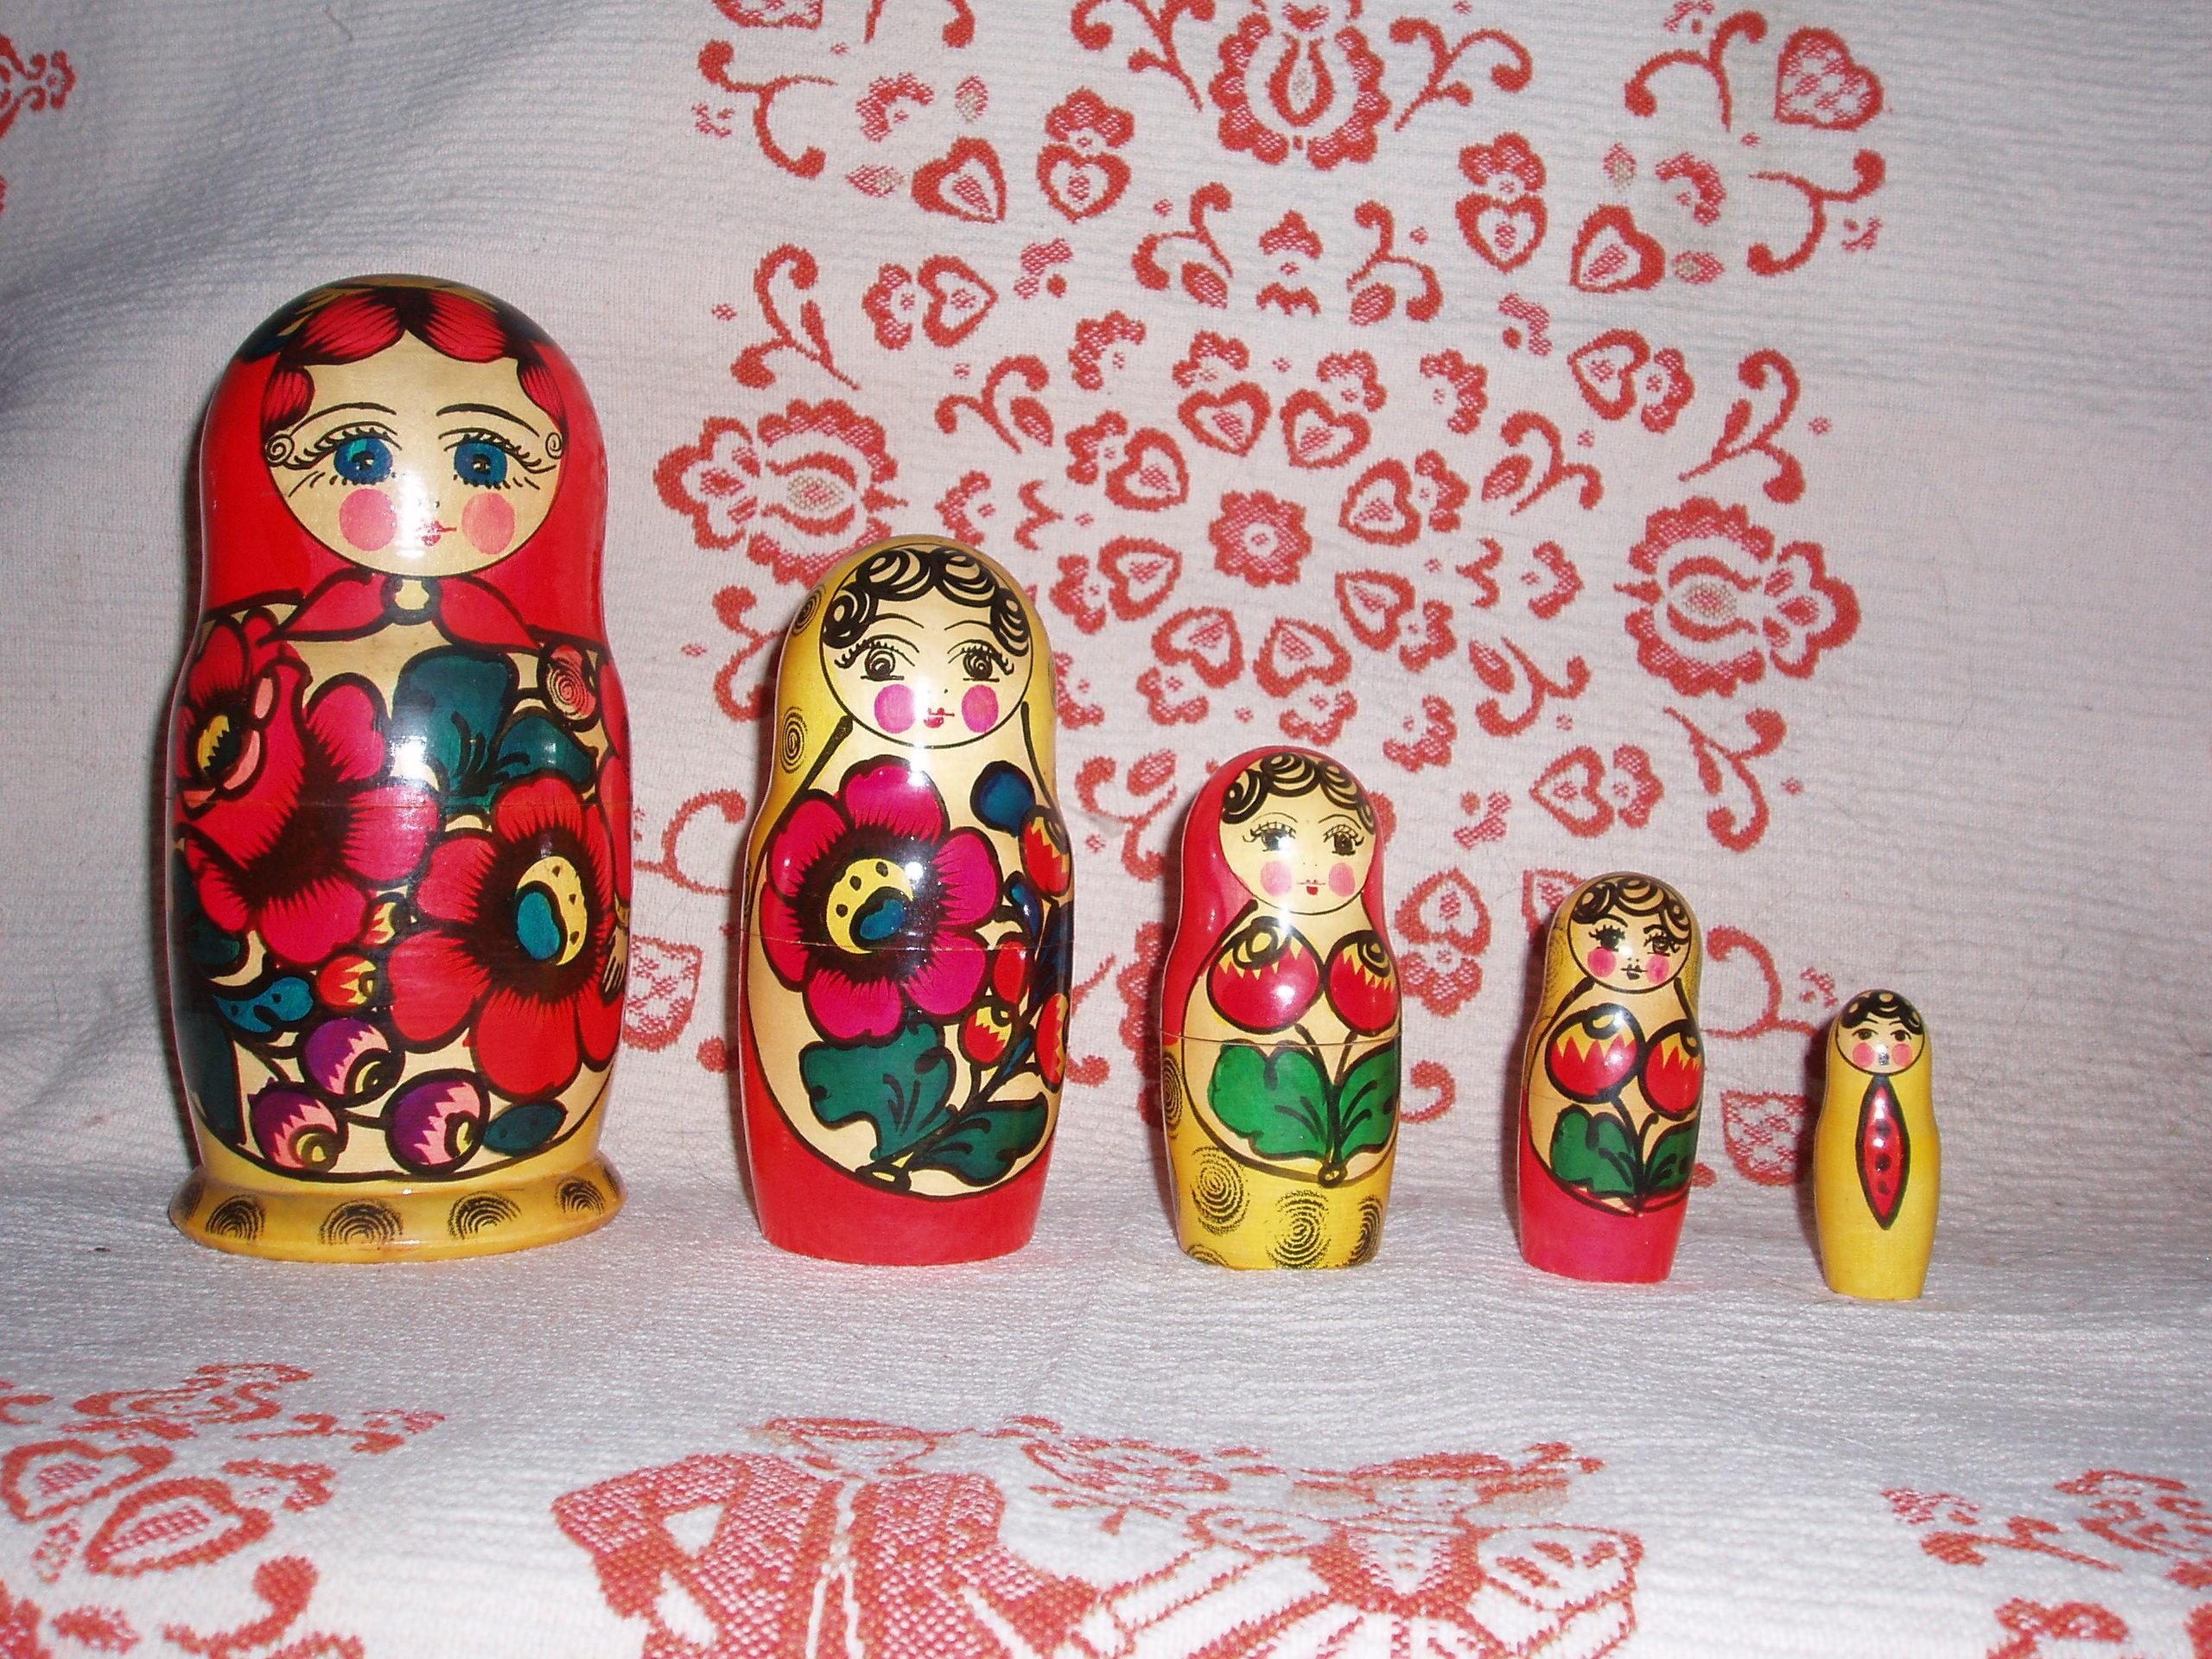
\includegraphics[width=0.5\textwidth]{Russian-Matroshka.jpg}
    \caption{Russian nesting dolls.}
    \label{rnd}
\end{figure}

The $i^{th}$ nesting doll has a maximum weight of $w_i$ and maximum value of $v_i$.
However, these particular dolls are unique, i.e., they are infinitely decomposable. 
In other words, if $x_i$ is the normalized amount of the doll that we can take, we can take any fraction of the nesting doll $x_i \in [0,1]$.
For example, $x_i=1$ would mean that we take the whole doll and all infinitesimally small dolls incurring a weight of $w_i$ and adding value $v_i$.
Whereas, if $x_i=[0,1)$ we would take the fractional amount $x_i$ of $w_i$, incur a weight of $x_i w_i$ and adding value $x_i v_i$.

Derek has a backpack with a capacity of $Z$, meaning that the sum of the items he takes must weigh less than $Z$
\begin{equation}
    \sum_i x_i w_i \leq Z
\end{equation}
and he wants to select the weights for each item such that his total profits 
\begin{equation}
   \sum_{i} x_i v_i
\end{equation}
are maximized.

Develop a greedy algorithm to set the $x_i$ values optimally, i.e., maximizing Derek's profits.
Prove your algorithm is correct.

\subsection*{Solution}

The greedy solution for this problem is quite simple and intuitive:

\begin{enumerate}
    \item Find the item with the greatest value-per-weight ratio.
    \item Add as much of that item as possible to the backpack.
    \item Repeat with all remaining items until the backpack is full.
\end{enumerate}

\begin{thm}
    The selection algorithm outlined above produces the most valuable selection of items.
\end{thm}

\begin{proof}
    Let $d_i$ be the item with the maximum value-to-weight ratio, we must then show that the optimal solution contains the maximum possible amount of $d_i$ in order to prove our algorithm's correctness. We can prove this statement by disproving it's converse; that there is an optimal solution that did not take the maximum amount of $d_i$, and that the backpack is full at the end.

    $\hfill \break$
    Due to the fact that $d_i$ is known to have the highest value-to-weight ratio in the set, there must exist a doll $d_j$ such that $\frac{v_j}{w_j} < \frac{v_i}{w_i}$. Since we know that the dolls are infinitely decomposable, we know that we can replace a quantity of $d_j$ that weighs $x$ weight, with $d_i$ of the same weight and receive a higher total value. 
    
    $\hfill \break$
    In this way, there will always be a scenario in which the maximum value-to-weight ratio doll (within the capacity limits) must be included in the optimal solution. As such, we have disproven our supposition since the optimal solution does not contain the maximum amount of $d_i$ that it is able to, and as such it is not optimal.
\end{proof}

\newpage
\section*{Problem 2 -- Min-cuts (15\%)}

Let $A$ and $B$ be a partition of the nodes of $G(V,E)$ such that $s \in $A and $t \in B$.
The capacity of a cut denoted $c(A,B)$, is the sum of the capacities out of $A$.
Enumerate \textit{all} the minimum $s-t$ cuts in the flow networks in Figures~\ref{flow1} and \ref{flow2}; give their value.

\begin{figure}[h!]
    \centering
    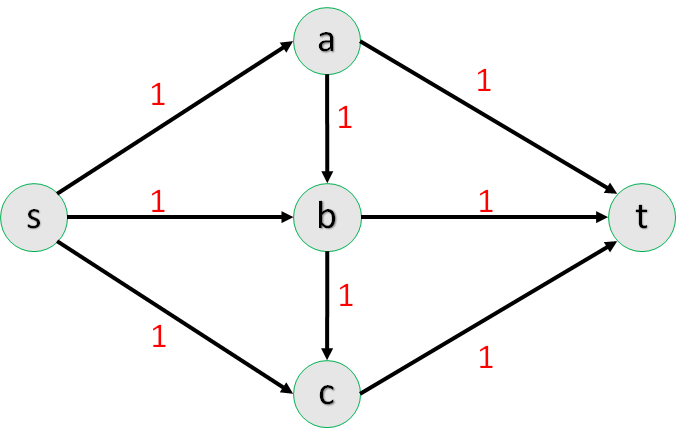
\includegraphics[width=0.5\textwidth]{flow1.png}
    \caption{Flow graph 1. The capacities are labeled on the edges.}
    \label{flow1}
\end{figure}

\begin{figure}[h!]
    \centering
    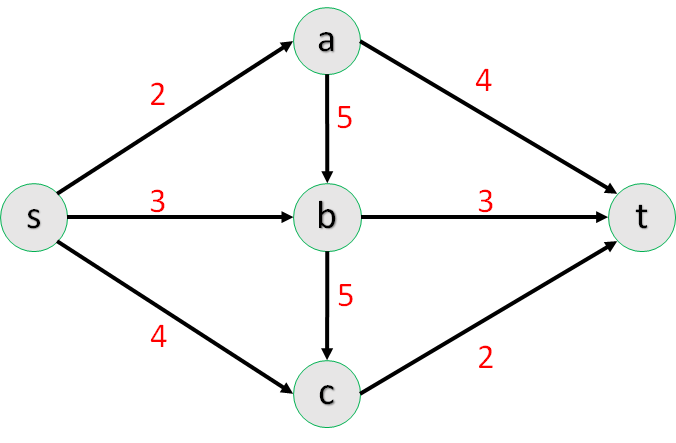
\includegraphics[width=0.5\textwidth]{flow2.png}
    \caption{Flow graph 2. The capacities are labeled on the edges.}
    \label{flow2}
\end{figure}

\newpage
\subsection*{Solution}

\subsubsection*{Part 1}

In Figure 2, we can see the following from the given network graph:

\begin{itemize}
    \item $s$ has $flow_{out} = 1$ into $a, b, c$ which creates a total flow of \textit{three}.
    \item $a$ has $flow_{in} = 1$ from $s$, and itself has $flow_{out} = 1$ to $b, t$.
    \item $b$ has $flow_{in} = 1$ from $a$ and $s$, and itself has $flow_{out} = 1$ to $c, t$.
    \item $c$ has $flow_{in} = 1$ from $b$ and $s$, and itself has $flow_{out} = 1$ to $t$.
    \item $t$ has $flow_{in} = 1$ from all $a, b, c$ which creates a total flow of \textit{three}.
\end{itemize}

In this way, since all edges in the network have the same weight, we can assume that the minimum-cut is \textit{three}.

\subsubsection*{Figure 3}

In Figure 3, we can see the following from the given network graph:

\begin{itemize}
    \item $s$ has $flow_{out} = 2, 3, 4$ into $a, b, c$ respectively; this creates a total flow of \textit{nine}.
    \item $a$ has $flow_{in} = 2$ from $s$, and itself has $flow_{out} = 5, 4$ to $b, t$ respectively.
    \item $b$ has $flow_{in} = 3, 5$ from $s$ and $a$ respectively, and itself has $flow_{out} = 5, 3$ to $c, t$ respectively.
    \item $c$ has $flow_{in} = 4, 5$ from $s$ and $b$ respectively, and itself has $flow_{out} = 2$ to $t$.
    \item $t$ has $flow_{in} = 4, 3, 2$ from $a, b, c$ respectively, which creates a total flow of \textit{nine}.
\end{itemize}

In this way, we would receive cuts of 2, 3, and 2 respectively, and would have an overall minimum-cut of \textit{seven}. 

\newpage
\section*{Problem 3 -- Reducing problems to flow (15\%)}

\begin{enumerate}
    \item Let figure \ref{flow2} represent a company's transportation network from the factory (source) to the warehouse (sink), and the capacity of the roads in between intermediate cities (a, b, and c).
    Recently, the company has decided to expand and build more factories and warehouses.
    Their new flow network is shown in Figure~\ref{flow3}.
    Modify Figure~\ref{flow3} to allow the new network to be solved with the single source, single sink Ford-Fulkerson algorithm.
    \item Consider a different formulation of the hospital-resident matching problem that is arguably closer to reality.
We have $n$ hospitals and $m$ residents.
Each resident $r \in R$ selects $3$ hospitals $h \in H$ that are acceptable; we assume that a hospital will accept any resident.
A matching $M$ in G is a subset of edges such that each node appears in at most one edge in $M$.

Give a polynomial-time algorithm to find an $M$ with maximum cardinality.
For this problem, you need to translate the text into a mathematical formulation, so define the data structures you use to model the problem.
If you make assumptions, make sure you state them.
You do not need to prove the runtime but justify why it is correct.
Finally, what is the value of the maximum flow?


\end{enumerate}

\begin{figure}[h!]
    \centering
    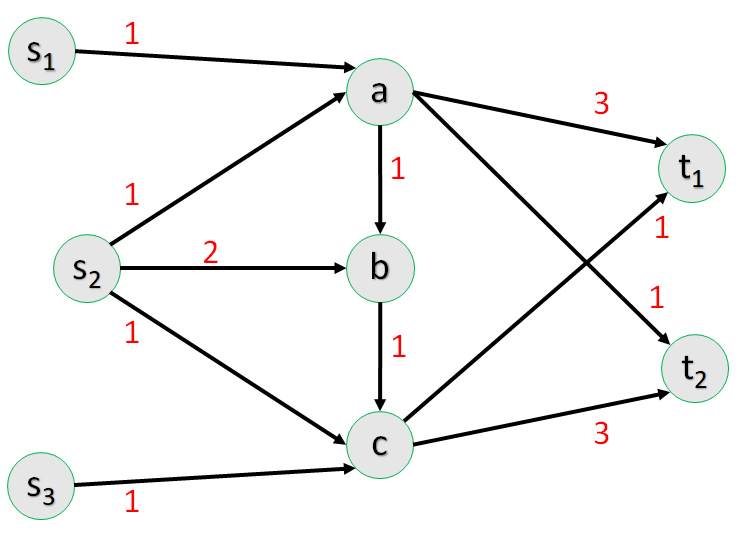
\includegraphics[width=0.5\textwidth]{flow3.png}
    \caption{A company expanding its business. The capacities are labeled on the edges.}
    \label{flow3}
\end{figure}

\newpage
\subsection*{Solution}

\subsubsection*{Part 1}

\begin{figure}[!htb]
    \centering
    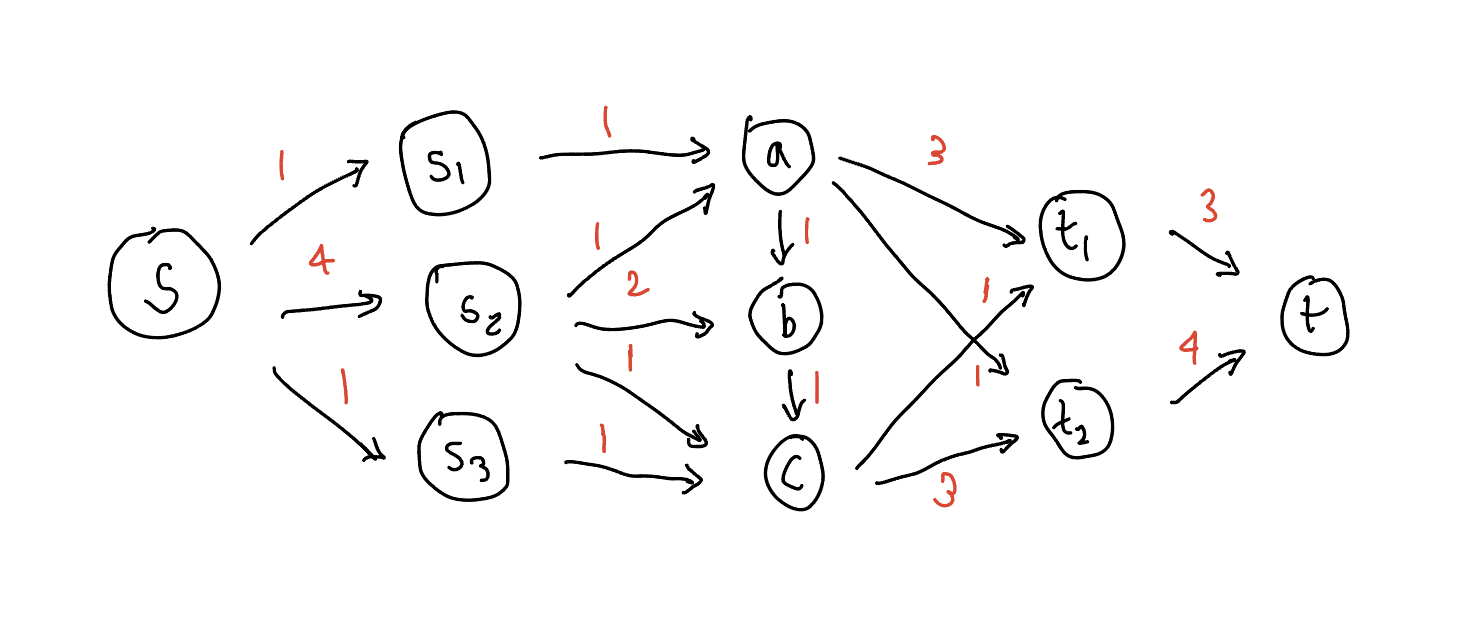
\includegraphics[height=2.5in]{q3-1.jpeg}
    \caption{Modified Network Graph with One Source and One Sink}
    \label{q3-1}
\end{figure}

\subsubsection*{Part 2}

We can conduct the same procedures used to solve Part 1, in which we prepend a source node that feeds into all of the residents, and a sink node that feeds from all of the hospitals. Once these nodes are added, we can add edges from each resident to each hospital, each with a capacity of one. Pursuant to the problem statement, we must add an edge from each hospital to the sink node, each with a capacity of three.

$\hfill \break$
Once the network flow is setup accordingly, we can see that the minimum-cut of the network would in turn be the maximum flow of the network, and the maximum cardinality matching. In order to actually find the value of the maximum flow for this problem, we can utilize the Ford-Fulkerson algorithm, which has a polynomial runtime of $O(VE^2)$, where $V$ refers to the number of vertices, and $E$ refers to the number of edges in the network.

$\hfill \break$
In order to implement the Ford-Fulkerson algorithm, we must first initialize the flow to zero, and then we must find an augmenting path from the source to the sink. If such a path exists, we must then find the minimum capacity of the edges in the path, and then add that value to the flow. We must then update the residual graph, and repeat the process until no augmenting path exists. Once this is done, we can return the flow value, which will be the maximum flow of the network.

\end{document}
